% abtex2-modelo-artigo.tex, v-1.9.2 laurocesar
% Copyright 2012-2014 by abnTeX2 group at http://abntex2.googlecode.com/ 
%

% ------------------------------------------------------------------------
% ------------------------------------------------------------------------
% abnTeX2: Modelo de Artigo Acadêmico em conformidade com
% ABNT NBR 6022:2003: Informação e documentação - Artigo em publicação 
% periódica científica impressa - Apresentação
% ------------------------------------------------------------------------
% ------------------------------------------------------------------------

\documentclass[
% -- opções da classe memoir --
article,			% indica que é um artigo acadêmico
11pt,				% tamanho da fonte
oneside,			% para impressão apenas no verso. Oposto a twoside
a4paper,			% tamanho do papel. 
% -- opções da classe abntex2 --
%chapter=TITLE,		% títulos de capítulos convertidos em letras maiúsculas
%section=TITLE,		% títulos de seções convertidos em letras maiúsculas
%subsection=TITLE,	% títulos de subseções convertidos em letras maiúsculas
%subsubsection=TITLE % títulos de subsubseções convertidos em letras maiúsculas
% -- opções do pacote babel --
english,			% idioma adicional para hifenização
brazil,				% o último idioma é o principal do documento
sumario=tradicional
]{abntex2}


% ---
% PACOTES
% ---

% ---
% Pacotes fundamentais 
% ---
\usepackage{lmodern}			% Usa a fonte Latin Modern
\usepackage[T1]{fontenc}		% Selecao de codigos de fonte.
\usepackage[utf8]{inputenc}		% Codificacao do documento (conversão automática dos acentos)
\usepackage{indentfirst}		% Indenta o primeiro parágrafo de cada seção.
\usepackage{nomencl} 			% Lista de simbolos
\usepackage{color}				% Controle das cores
\usepackage{graphicx}			% Inclusão de gráficos
\usepackage{float}
\usepackage{microtype} 			% para melhorias de justificação

% ---

% ---
% Pacotes adicionais, usados apenas no âmbito do Modelo Canônico do abnteX2
% ---
\usepackage{lipsum}				% para geração de dummy text
% ---

% ---
% Pacotes de citações
% ---
\usepackage[brazilian,hyperpageref]{backref}	 % Paginas com as citações na bibl
\usepackage[alf]{abntex2cite}	% Citações padrão ABNT
% ---

% ---
% Informações de dados para CAPA e FOLHA DE ROSTO
% ---
\titulo{Atividade VI }
\autor{ Rafael Gonçalves de Oliveira Viana}
\local{Brasil}
\data{2017}
% ---

% ---
% Configurações de aparência do PDF final

% alterando o aspecto da cor azul
\definecolor{blue}{RGB}{41,5,195}

% informações do PDF
\makeatletter
\hypersetup{
	%pagebackref=true,
	pdftitle={\@title}, 
	pdfauthor={\@author},
	pdfsubject={Artigo},
	pdfcreator={LaTeX with abnTeX2},
	pdfkeywords={abnt}{latex}{abntex}{abntex2}{atigo científico}, 
	colorlinks=true,       		% false: boxed links; true: colored links
	linkcolor=blue,          	% color of internal links
	citecolor=blue,        		% color of links to bibliography
	filecolor=magenta,      		% color of file links
	urlcolor=blue,
	bookmarksdepth=4
}
\makeatother
% --- 

% ---
% compila o indice
% ---
\makeindex
% ---

% ---
% Altera as margens padrões
% ---
\setlrmarginsandblock{3cm}{3cm}{*}
\setulmarginsandblock{3cm}{3cm}{*}
\checkandfixthelayout
% ---

% --- 
% Espaçamentos entre linhas e parágrafos 
% --- 

% O tamanho do parágrafo é dado por:
\setlength{\parindent}{1.3cm}

% Controle do espaçamento entre um parágrafo e outro:
\setlength{\parskip}{0.2cm}  % tente também \onelineskip

% Espaçamento simples
\SingleSpacing

% ----
% Início do documento
% ----
\begin{document}
	
	% Retira espaço extra obsoleto entre as frases.
	\frenchspacing 
	
	% ----------------------------------------------------------
	% ELEMENTOS PRÉ-TEXTUAIS
	% ----------------------------------------------------------
	
	%---
	%
	% Se desejar escrever o artigo em duas colunas, descomente a linha abaixo
	% e a linha com o texto ``FIM DE ARTIGO EM DUAS COLUNAS''.
	% \twocolumn[    		% INICIO DE ARTIGO EM DUAS COLUNAS
	%
	%---
	% página de titulo
	\maketitle
	\begin{enumerate}
		\item Crie uma view que informe o quanto cada instrutor
		arrecadou.
				\begin{verbatim}
create or replace view arrecadou as select i.cod_instrutor, i.nome_instrutor,
sum(t.preco_hora_instrutor*c.carga_horaria) arrecadado from
instrutores i, turmas t, cursos c 
where i.cod_instrutor = t.cod_instrutor AND
c.cod_curso = t.cod_curso AND
t.preco_hora_instrutor <> 0 group 
by i.nome_instrutor, i.cod_instrutor  order by arrecadado;
				\end{verbatim}
				
				\begin{center}
					\begin{figure}[H]
						\centering
						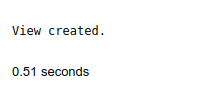
\includegraphics[scale=0.5]{./imagens/at-01.png}
						\caption{View criada.}
						\label{rota-1}
					\end{figure}
				\end{center}
				\begin{verbatim}
		select * from arrecadou;
			\end{verbatim}
			
				\begin{center}
				\begin{figure}[H]
					\centering
					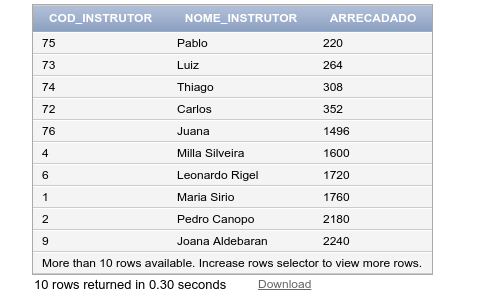
\includegraphics[scale=0.5]{./imagens/at-02.png}
					\caption{View selecionada.}
					\label{rota-1}
				\end{figure}
			\end{center}
			
						\item  Monte uma view que revele alunos, cursos e total
						pago por cada um.
						\begin{verbatim}

		create or replace view pagamento as
		select a.nome_aluno, c.nome_curso, sum(c.preco) total
		from alunos a, cursos c, historico h, turmas t
		where a.matricula = h.matricula and 
		h.cod_turma = t.cod_turma and
		c.cod_curso = t.cod_curso
		group by a.nome_aluno, c.nome_curso
		having sum(c.preco)>0;
						\end{verbatim}
						
						\begin{center}
							\begin{figure}[H]
								\centering
								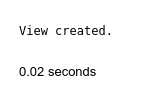
\includegraphics[scale=0.5]{./imagens/at-03.png}
								\caption{View criada.}
								\label{rota-1}
							\end{figure}
						\end{center}
					
					
				   \begin{verbatim}
					
					select * from pagamento ;
					\end{verbatim}
					
						
					\begin{center}
						\begin{figure}[H]
							\centering
							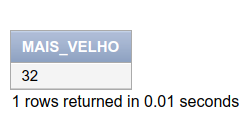
\includegraphics[scale=0.5]{./imagens/at-04.png}
							\caption{View selecionada.}
							\label{rota-1}
						\end{figure}
					\end{center}
					
						\item
						 Faça uma view que mostre a média vendida por
						curso.
					\begin{verbatim}
			create or replace view media_vendida as select
			c.nome_curso Curso, avg(preco) mediaVendida from 
			cursos c, turmas t where c.cod_curso = t.cod_curso 
			group by c.nome_curso having avg(preco) > 0;
					\end{verbatim}
							\begin{center}
							\begin{figure}[H]
								\centering
								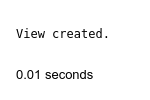
\includegraphics[scale=0.5]{./imagens/at-05.png}
								\caption{View criada.}
								\label{rota-1}
							\end{figure}
						\end{center}
							\begin{verbatim}
					 select * from media_vendida;
						\end{verbatim}
						\begin{center}
							\begin{figure}[H]
								\centering
								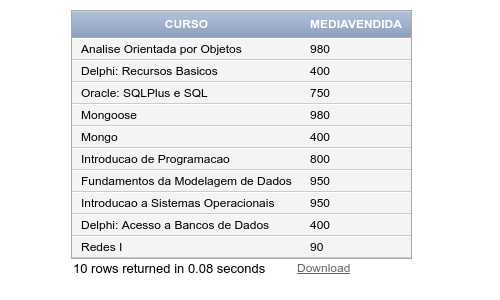
\includegraphics[scale=0.5]{./imagens/at-06.png}
								\caption{View selecionada.}
								\label{rota-1}
							\end{figure}
						\end{center}
				
								\item
								Monte uma view que sirva como base para a lista
								de presenças. Devem constar: nome do aluno,
								nome do curso, carga horária, nome do instrutor e
								sala.
						\begin{verbatim}
					create or replace view lista_presenca
					as select a.nome_aluno Aluno, c.nome_curso Curso, c.carga_horaria,
					i.nome_instrutor, t.sala from alunos a, instrutores i, cursos c, turmas t,
					historico h where a.matricula = h.matricula and h.cod_turma =
			t.cod_turma and  i.cod_instrutor = t.cod_instrutor and c.cod_curso = 
			t.cod_curso order by a.nome_aluno;
					
						\end{verbatim}
						\begin{center}
							\begin{figure}[H]
								\centering
								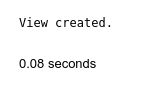
\includegraphics[scale=0.5]{./imagens/at-07.png}
								\caption{View criada.}
								\label{rota-1}
							\end{figure}
						\end{center}
						\begin{verbatim}
				select * from lista_presenca ;
						\end{verbatim}
						\begin{center}
							\begin{figure}[H]
								\centering
								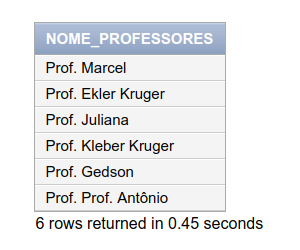
\includegraphics[scale=0.5]{./imagens/at-08.png}
								\caption{View selecionada.}
								\label{rota-1}
							\end{figure}
						\end{center}
						
	\end{enumerate}				
			
\end{document}
